% !TEX encoding = UTF-8
% !TEX TS-program = pdflatex
% !TEX root = ../../tesi.tex

\section{Strumenti e configurazione}
Inizialmente, prima di Iniziare la fase di sviluppo, ho svolto un processo di organizzazione e configurazione degli strumenti per procede al meglio con la fase successiva. 

\subsection{Strumenti di gestione del progetto}
Descrizione degli strumenti utilizzati per la gestione del progetto.

\subsection{Documentazione}
Per quanto riguarda la scrittura della documentazione e la realizzazione dei vari diagrammi UML, ho utilizzato, rispettivamente, il linguaggio Markdown e Mermaid. Markdown è un linguaggio di \textit{markup} con una sintassi del testo semplice progettata in modo che possa essere convertita in HTML. È perfettamente integrabile con la piattaforma GitHub, la quale mette a disposizione la lettura online dei documenti scritti in Markdown.
Mermaid, invece, è uno strumento che permette di generare le immagini dei diagrammi UML a partire da un \textit{file} con estensione mmd. Questo ha facilitato di molto la realizzazione dei diagrammi richiesti, senza doversi occupare della parte grafica. In seguito le immagini generate sono state importate dentro il documento in scritto in Markdown.

\subsection{Ambiente di sviluppo}
Come ambiente di sviluppo sono stati utilizzati IntelliJ Idea per lo sviluppo di codice che riguardava il linguaggio Java e VS Code per quello che riguardava Solidity.
IntelliJ IDEA è un ambiente di sviluppo integrato per il linguaggio di programmazione Java. Ha molte funzionalità che facilitano la gestione del codice, infatti esegue automaticamente il \textit{code refactoring} in base alle modifiche che si vogliono apportare, si integra perfettamente con lo strumento di versionamento GIT e gli strumenti di \textit{build automation} maven e gradle.
VS Code, invece, è un code editor sviluppato su Electron, un \textit{framework} attraverso il quale è possibile sviluppare applicazioni \textit{desktop} utilizzando le tecnologie web. Appena installato non ha molte funzionalità, ma grazie alle numerose estensioni che sono state create, è possibile arrivare considerarlo anche un IDE. Principalmente è stato utilizzato per lo sviluppo in Solidity, con estensioni che avviassero lo strumento di \textit{lint} e formattazione del codice ad ogni salvataggio.

\subsection{Tecnologie usate}
Descrizione dei vari linguaggi di programmazione, framework, librerie e strumenti di build automation.

\paragraph{Java} 
Java è uno dei linguaggi più utilizzati al mondo. È un linguaggio di programmazione ad alto livello, orientato agli oggetti e a tipizzazione statica. In questo progetto è stato utilizzato per lo sviluppo della libreria per l'integrazione con il \textit{back-end}, visto che quest'ultimo è stato sviluppato utilizzando il \textit{framework} Spring. 

\paragraph{Solidity}
Solidity è un linguaggio di programmazione orientato agli oggetti per la scrittura di \textit{smart contract}. Può essere utilizzato su varie piattaforme \textit{blockchain}, ma quella più famosa e originale, per cui è stato creato, è Ethereum. Come Java, Solidity non viene tradotto in linguaggio macchina ma, per il fatto che ogni \textit{smart contract} deve essere separato dall'ambiente su cui gira, viene tradotto in \textit{bytecode} ed eseguito dalla \textit{EVM} (\textit{Ethereum Virtual Machine}).

\paragraph{Takamaka}
Takamaka è un \textit{subset} di Java, ovvero un sottoinsieme della sintassi del linguaggio Java, utilizzato per la scrittura di Smart Contract per nella \textit{blockchain} Hotmoka.

% \paragraph{Typescript}
% Typescript è un \textit{superset} di Javascript, al quale aggiunge la tipizzazione statica del codice, una sintassi più aggiornata per la scrittura delle classi e delle interfacce e molti altri costrutti che facilitano la scrittura del codice. In questo progetto 

\paragraph{HardHat}
HardHat è un ambiente di sviluppo per \textit{smart contract} in Solidity per Ethereum. Ha vari strumenti che facilitano di molto lo sviluppo ed i più importanti sono i seguenti:
\begin{itemize}
  \item possibilità di utilizzo di una \textit{blockchain} temporanea e relativi \textit{wallet}, la quale annulla il \textit{block time} togliendo qualsiasi forma di \textit{proof of X}, durante la fase di testing, in modo da velocizzarla;
  \item possibilità di scrivere vari script in Typescript per eseguire il \textit{deploy} dello \textit{smart contract}, oppure semplicemente per comunicare con uno precedentemente caricato, su varie reti Ethereum, come quella pubblica o una qualsiasi \textit{testnet}<
  \item possibilità di scrivere tutti i \textit{test} utilizzando Typescript;
  \item integrazione con lo strumento solcover per ottenere il report del code coverage raggiunto.
\end{itemize}

\paragraph{Ganache}
Ganache è uno strumento per creare una \textit{blockchain} locale non temporanea per poter svolgere vari test. Offre molte funzionalità, ma quella più importante è la possibilità di avere a disposizione moltissimi \textit{wallet}

\begin{figure}[h!]
  \centering
  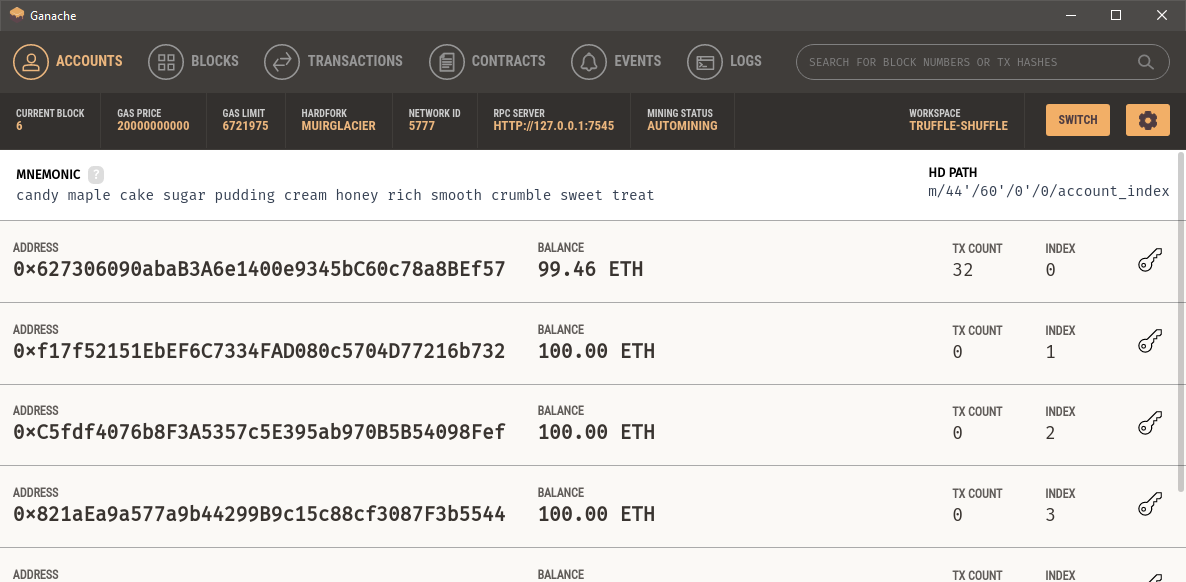
\includegraphics{capitolo3/ganache.png}
  \caption{Finestra dello strumento Ganache}
\end{figure}

\paragraph{Maven}
Maven è uno strumento di gestione di progetti \textit{software} basati su Java e \textit{build automation}. Effettua automaticamente il \textit{download} delle librerie Java e \textit{plug-in} Maven dai vari \textit{repository} definiti scaricandoli in locale. Questo permette di recuperare in modo uniforme i vari file \textit{JAR} e di poter spostare il progetto da un ambiente all'altro, avendo la sicurezza di utilizzare sempre le stesse versioni delle librerie. Utilizza file XML chiamato POM (\textit{Project Object Model}), dove vengono descritte le dipendenze tra il progetto e le varie versioni di librerie necessaire, nonchè le dipendenze fra di esse. È stato utilizzato per la gestione di tutti i progetti Java sviluppati durante il percorso di stage, ovvero la libreria per l'integrazione e gli \textit{smart contract} per HotMoka.

\paragraph{ERC721 OpenZeppelin}
Come implementazione dello standard \textit{ERC721}, è stata utilizzata quella più famosa e conosciuta nel mondo Ethereum, ovvero quella data dall'azienda OpenZeppelin. Oltre alla sua grande fama e al fatto che è utilizzata dalla maggior parte della \textit{community}, è stata scelta perché non ci sono vulnerabilità attualmente conosciute.

\paragraph{JUnit5}


\paragraph{Mockito}

\paragraph{Mocka}

\paragraph{Chai}

\paragraph{Solhint}

\paragraph{Checkstyle}


\subsection{Analisi statica del codice}
Descrizione degli strumenti utilizzati per l'automazione dell'analisi statica del codice.

\subsection{Way of working}
Spiegazione di come viene organizzato e gestito il flusso di sviluppo.
